\begin{tikzpicture}
\begin{axis}[
	name=plot1,
	axis y line=middle, axis x line=bottom,
	enlargelimits = false, clip=false,
	scale only axis,
	width=\textwidth,
	height=0.2\textwidth,
	ymin=-0.6,	ymax=0.6,
	xmin={0}, xmax={200},
	axis line style={->,>=stealth},
	x axis line style={shorten >= -0.25cm}, 
	xlabel={\large $t$ (ms)},
	ylabel={\large $x(t)$},
	every axis x label/.style={
		at={(ticklabel* cs:1)},
		xshift=0.5cm,
		anchor=north west,
	},
	every axis y label/.style={
		at={(ticklabel* cs:1)},
		anchor=south,
	},
	xtick={50,100,...,200},
	xmajorgrids,
	ytick=\empty,
	extra x ticks={50,100,...,200},
	extra x tick labels={550, 1100,...,2200},
	every extra x tick/.style={major tick length=0pt,
	xtick align=outside,yshift=-15pt},
	every outer y axis line/.append style={white!15!black},
	every y tick label/.append style={font=\color{white!15!black}},
	legend style={draw=white!15!black,fill=white,legend cell align=left}]
	\node[below, anchor=north west, xshift=0.5cm,yshift=-15pt]  at (axis cs: 200,-0.6) {\large $n$ (samples)};
	
	\only<1-|handout:1->{
		\addplot [smooth, color=black, solid, line width=1pt] table[x index=0,y index=1] {figs/data/speech_sample.dat};
	}

	\only<2-|handout:2->{
		\addplot [smooth, color=blue2, solid, line width=1pt, restrict x to domain=0:63] table[x index=0,y index=1] {figs/data/speech_sample.dat};
	}

	\only<3-|handout:3->{
	\addplot [smooth, color=red2, solid, line width=1pt, restrict x to domain=50:113] table[x index=0,y index=1] {figs/data/speech_sample.dat};
	}

	\only<4-|handout:4->{
	\addplot [smooth, color=green2, solid, line width=1pt, restrict x to domain=100:163] table[x index=0,y index=1] {figs/data/speech_sample.dat};
	}

	\only<5-|handout:5->{
	\addplot [smooth, color=orange2, solid, line width=1pt, restrict x to domain=150:213] table[x index=0,y index=1] {figs/data/speech_sample.dat};
	}
	
\end{axis}

\begin{axis}[
name=plot2,
at=(plot1.below south east), anchor=above north east,
axis y line=middle, axis x line=bottom,
enlargelimits = false, clip=false,
scale only axis,
width=\textwidth,
height=0.2\textwidth,
%ymin=-0.6,	ymax=0.6,
xmin={0}, xmax={5.5},
axis line style={->,>=stealth},
x axis line style={shorten >= -0.25cm}, 
xlabel={\large Frequency (kHz)},
ylabel={\large dB},
every axis x label/.style={
	at={(ticklabel* cs:1)},
	xshift=0.5cm,
	anchor=north west,
},
every axis y label/.style={
	at={(ticklabel* cs:1)},
	anchor=south,
},
ymajorgrids,
xtick={0,..., 5},
every outer y axis line/.append style={white!15!black},
every y tick label/.append style={font=\color{white!15!black}},
legend style={draw=white!15!black,fill=white,legend cell align=left}]

\only<2|handout:2>{
	\addplot [smooth, color=blue2, solid, line width=1pt] table[x index=0,y index=4] {figs/data/speech_spectrogram_dft.dat};
}

\only<3|handout:3>{
	\addplot [smooth, color=red2, solid, line width=1pt] table[x index=0,y index=3] {figs/data/speech_spectrogram_dft.dat};
}

\only<4|handout:4>{
	\addplot [smooth, color=green2, solid, line width=1pt] table[x index=0,y index=2] {figs/data/speech_spectrogram_dft.dat};
}

\only<5|handout:5>{
	\addplot [smooth, color=orange2, solid, line width=1pt] table[x index=0,y index=1] {figs/data/speech_spectrogram_dft.dat};
}

\end{axis}

\onslide<2|handout:2>{
\node[anchor=north east] at ($(plot2.south east)+(0.8cm, -0.7cm)$) {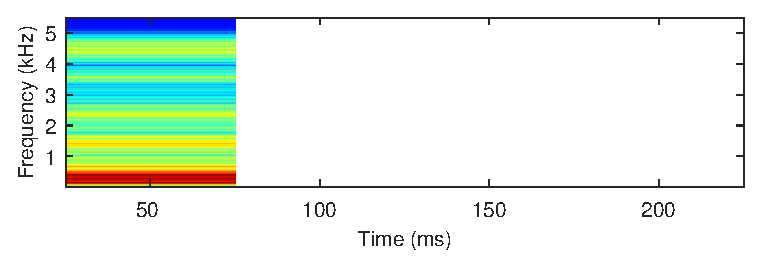
\includegraphics{figs/spectrogram_demo_pt1.eps}};
}

\onslide<3|handout:3>{
	\node[anchor=north east] at ($(plot2.south east)+(0.8cm, -0.7cm)$) {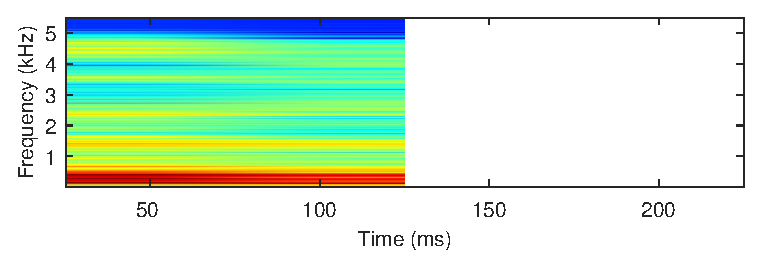
\includegraphics{figs/spectrogram_demo_pt2.eps}};
}

\onslide<4|handout:4>{
	\node[anchor=north east] at ($(plot2.south east)+(0.8cm, -0.7cm)$) {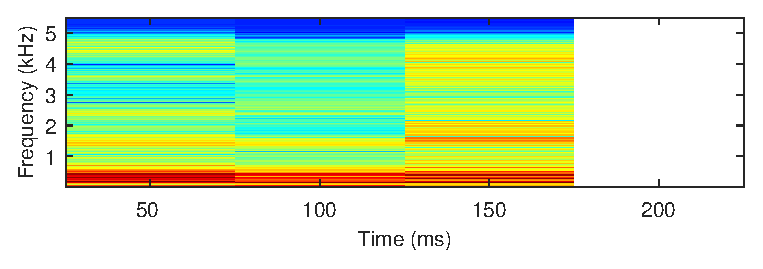
\includegraphics{figs/spectrogram_demo_pt3.eps}};
}

\onslide<5|handout:5>{
	\node[anchor=north east] at ($(plot2.south east)+(0.8cm, -0.7cm)$) {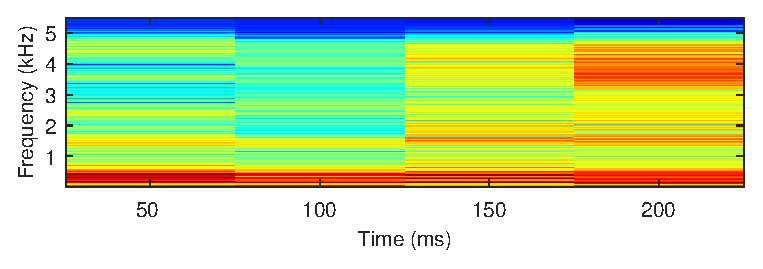
\includegraphics{figs/spectrogram_demo_pt4.eps}};
}

\end{tikzpicture}	
